\usetikzlibrary{positioning,arrows,shapes}
\section[Método Multipolar Rápido]{Método Multipolar Rápido (Fast Multipole Method -\ FMM)}\label{subsec:fmm}

El Método Multipolar Rápido (FMM), es una técnica computacional fundamental desarrollada para acelerar significativamente la evaluación de interacciones de largo alcance en sistemas de $N$ partículas o elementos~\cite{GreengardRokhlin1987, Martinsson2012}. Reconocido como uno de los algoritmos más influyentes del siglo XX~\cite{Cipra2000}, el FMM reduce drásticamente la complejidad computacional inherente a los problemas de $N$-cuerpos. Mientras que un cálculo directo de todas las interacciones par a par requiere $O(N^2)$ operaciones, el FMM logra esta tarea típicamente en $O(N)$ o $O(N \log N)$ operaciones, dependiendo de la distribución de las partículas y la variante del método empleada~\cite{BeatsonGreengard1997, GreengardRokhlin1987}. De manera más precisa, en $d$ dimensiones, la complejidad puede estimarse como $O(N \log^{(d-1)}(1/\epsilon))$ a medida que la precisión deseada $\epsilon$ tiende a cero~\cite{Martinsson2012}. Conceptualmente, el FMM puede interpretarse como un método para acelerar la multiplicación de un vector por una matriz densa específica que surge de la discretización de operadores integrales o sumas de interacciones par a par~\cite{ChenSF, Martinsson2012}.

\subsection{Principios Fundamentales y Funcionamiento}

El núcleo del FMM reside en una combinación de descomposición jerárquica del dominio computacional y el uso de expansiones matemáticas para aproximar interacciones~\cite{GreengardRokhlin1987}. El dominio se subdivide recursivamente mediante una estructura de árbol, como un \textit{quadtree} (2D) o un \textit{octree} (3D), agrupando las partículas o fuentes en celdas (o ``cajas'') a diferentes niveles de refinamiento~\cite{BeatsonGreengard1997, Martinsson2012}.

El método distingue entre interacciones de ``campo cercano'' y ``campo lejano''. Las interacciones entre partículas en celdas adyacentes (campo cercano) se calculan directamente, ya que las aproximaciones no son precisas a corta distancia~\cite{ChenSF, Ying2012}. Para las interacciones entre celdas bien separadas (campo lejano), el FMM emplea dos tipos principales de expansiones~\cite{GreengardRokhlin1987, Martinsson2012}:

\begin{itemize}
    \item \textbf{Expansión Multipolo (Saliente):} Representa el campo potencial generado por todas las fuentes \textit{dentro} de una celda (la ``fuente'') como una única serie convergente fuera de la celda. Esta expansión es válida a una distancia suficiente de la celda origen. Funciona como una representación compacta de las fuentes.
    \item \textbf{Expansión Local (Entrante):} Representa el potencial generado por fuentes \textit{distantes} (campo lejano) como una serie convergente \textit{dentro} de una celda (la ``objetivo''). Funciona como una representación compacta del campo externo que actúa sobre la celda.
\end{itemize}

El algoritmo clásico opera en dos fases principales sobre la estructura de árbol~\cite{BeatsonGreengard1997, GreengardRokhlin1987, Martinsson2012}:

\begin{itemize}
    \item \textbf{Paso Ascendente (Upward Pass):} Se calculan las expansiones multipolares para todas las celdas. Para las celdas hoja (el nivel más fino), se calcula directamente a partir de las fuentes contenidas. Para celdas padre, las expansiones se obtienen combinando (transladando y sumando) las expansiones de sus celdas hijas (operador \textit{Multipole-to-Multipole} o M2M).
    \item \textbf{Paso Descendente (Downward Pass):} Se calculan las expansiones locales para todas las celdas. Para cada celda, se convierten las expansiones multipolares de las celdas en su ``lista de interacción'' (celdas bien separadas en el mismo nivel, cuyos padres son vecinos pero ellas no) en contribuciones a su propia expansión local (operador \textit{Multipole-to-Local} o M2L). Luego, las expansiones locales de una celda padre se trasladan y se añaden a las expansiones locales de sus celdas hijas (operador \textit{Local-to-Local} o L2L).
\end{itemize}

Finalmente, en las celdas hoja, el potencial total en cada punto se calcula sumando la contribución directa de las fuentes en celdas vecinas y evaluando la expansión local acumulada (que representa todo el campo lejano). La clave de la eficiencia $O(N)$ radica en que el número de celdas en la lista de interacción es acotado (independiente de $N$), y las operaciones de traslación (M2M, M2L, L2L) tienen un coste que depende del orden de la expansión $p$ (relacionado con la precisión $\epsilon$) pero no de $N$~\cite{GreengardRokhlin1987}.

Desde una perspectiva matricial, el FMM explota la propiedad de que los bloques fuera de la diagonal de la matriz de interacción (que representan interacciones entre grupos de puntos separados espacialmente) tienen bajo rango numérico y pueden aproximarse eficientemente mediante factorizaciones de bajo rango, como las implícitas en las expansiones multipolares y locales~\cite{ChenSF, Martinsson2012}.

% --- Placeholder para Figura 1 (Jerarquía y Listas) ---
\begin{figure}[H]
    \centering
    % Descomenta la siguiente línea e inserta la ruta a tu imagen
    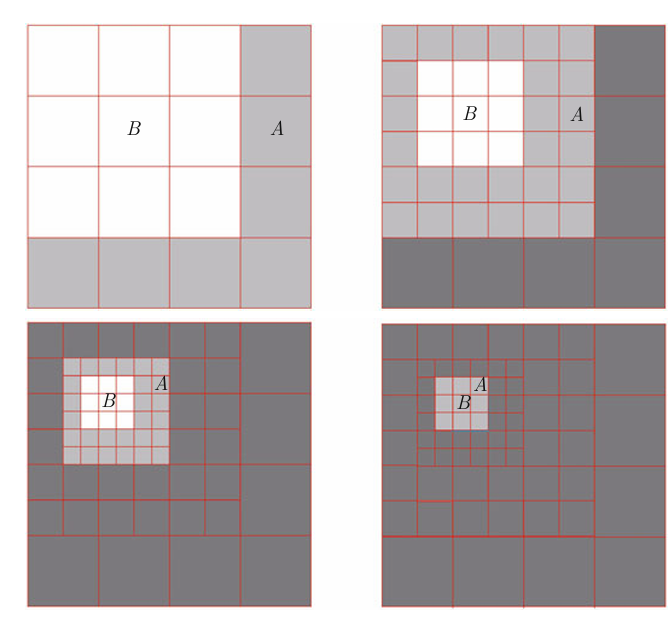
\includegraphics[width=0.65\textwidth]{img/marcoTeorico/fmm_esquema.png}
    %\fbox{\parbox{0.8\textwidth}{\centering Placeholder: Figura Esquema de la Jerarquía de Celdas y Listas de Interacción}}
    \caption{Esquema de la estructura jerárquica de celdas (e.g., quadtree) y la distinción entre interacciones de campo cercano (directas) y campo lejano (aproximadas mediante expansiones), incluyendo la lista de interacción. Adaptado de~\cite{GreengardRokhlin1987, Ying2012}.}%
    \label{fig:fmm_hierarchy}
\end{figure}

% --- Placeholder para Figura 2 (Operadores) ---
\begin{figure}[H]
    \centering
    \resizebox{0.85\textwidth}{!}{ % Cambia el factor de escala aquí
    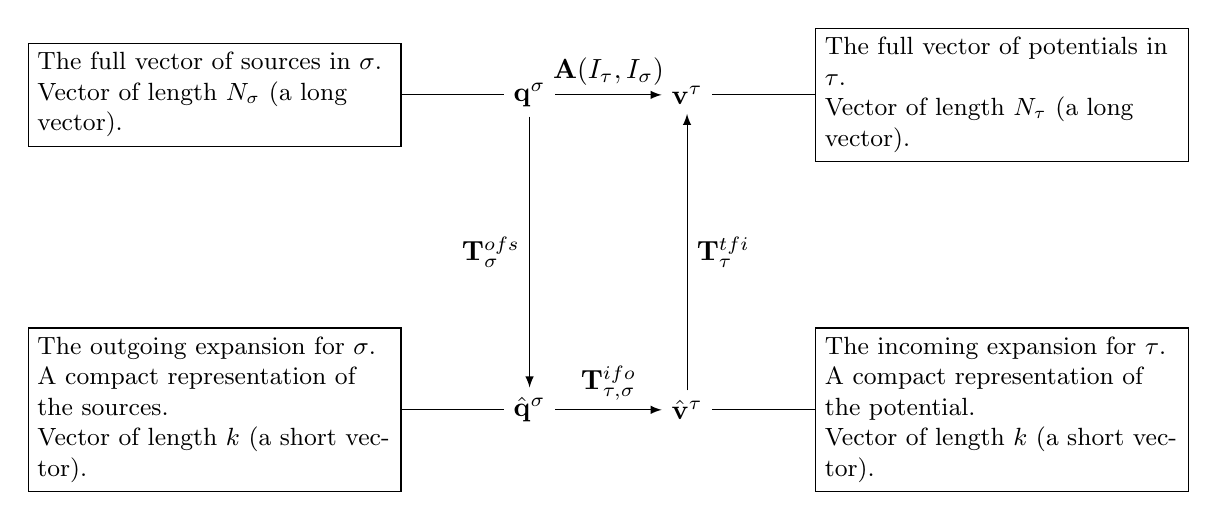
\begin{tikzpicture}[node distance=3cm and 4cm]
        % Define nodes for the vectors
        \node[draw, text width=4.5cm, align=left, font=\small] (q) at (-4, 2) {The full vector of sources in $\sigma$.\\ Vector of length $N_\sigma$ (a long vector).};
        \node[draw, text width=4.5cm, align=left, font=\small] (v) at (6, 2) {The full vector of potentials in $\tau$.\\ Vector of length $N_\tau$ (a long vector).};
        \node[draw, text width=4.5cm, align=left, font=\small] (qhat) at (-4, -2) {The outgoing expansion for $\sigma$.\\ A compact representation of the sources.\\ Vector of length $k$ (a short vector).};
        \node[draw, text width=4.5cm, align=left, font=\small] (vhat) at (6, -2) {The incoming expansion for $\tau$.\\ A compact representation of the potential.\\ Vector of length $k$ (a short vector).};

        % Define intermediate nodes
        \node (qmid) at (0, 2) {$\mathbf{q}^\sigma$};
        \node (vmid) at (2, 2) {$\mathbf{v}^\tau$};
        \node (qhatmid) at (0, -2) {$\hat{\mathbf{q}}^\sigma$};
        \node (vhatmid) at (2, -2) {$\hat{\mathbf{v}}^\tau$};

        % Draw arrows
        \draw[-latex] (qmid) -- (vmid) node[midway, above] {$\mathbf{A}(I_\tau, I_\sigma)$};
        \draw[-latex] (qmid) -- (qhatmid) node[midway, left] {$\mathbf{T}_\sigma^{\text{ofs}}$};
        \draw[-latex] (qhatmid) -- (vhatmid) node[midway, above] {$\mathbf{T}_{\tau,\sigma}^{\text{ifo}}$};
        \draw[-latex] (vhatmid) -- (vmid) node[midway, right] {$\mathbf{T}_\tau^{\text{tfi}}$};

        % Draw lines from boxes to intermediate nodes
        \draw (q) -- (qmid);
        \draw (v) -- (vmid);
        \draw (qhat) -- (qhatmid);
        \draw (vhat) -- (vhatmid);
    \end{tikzpicture}
    }
    \caption{Ilustración del flujo de información en el FMM:\ fuentes originales ($\mathbf{q}^\sigma$) $\rightarrow$ expansión saliente ($\hat{\mathbf{q}}^\sigma$) $\rightarrow$ expansión entrante ($\hat{\mathbf{v}}^\tau$) $\rightarrow$ potenciales ($\mathbf{v}^\tau$), mostrando los operadores T\textsuperscript{ofs}, T\textsuperscript{ifo}, y T\textsuperscript{tfi}. Adaptado de~\cite{Martinsson2012}.}%
    \label{fig:fmm_translations}
\end{figure}


\subsection{Contexto Histórico/Origen}

El FMM fue introducido formalmente por Leslie Greengard y Vladimir Rokhlin en su seminal artículo de 1987~\cite{GreengardRokhlin1987}, aunque ideas relacionadas con expansiones multipolares y métodos jerárquicos existían previamente (e.g.,~\cite{Appel1985, BarnesHut1986}). El trabajo de Greengard y Rokhlin proporcionó un marco riguroso y un algoritmo con complejidad demostrada de $O(N)$ para el problema de Laplace, revolucionando la simulación de $N$-cuerpos y la solución de ecuaciones integrales~\cite{GreengardRokhlin1987}. Su impacto fue tal que fue incluido en la lista de los 10 algoritmos más importantes del siglo XX~\cite{Cipra2000}.

\subsection{Variantes o Enfoques Principales}

El FMM ha evolucionado considerablemente desde su concepción original:
\begin{itemize}
    \item \textbf{Extensiones a otros Kernels:} Aunque inicialmente formulado para el kernel de Laplace ($1/r$), se ha extendido a otros kernels importantes como el de Helmholtz (ondas), Stokes (fluidos), Yukawa (física de partículas) y elasticidad~\cite{ChengEtAl1999, Martinsson2012, Rokhlin1990}. Para kernels oscilatorios como el de Helmholtz, se requieren enfoques más sofisticados (e.g., \textit{FMM direccional}) para mantener la eficiencia, especialmente a altas frecuencias~\cite{EngquistYing2009, Rokhlin1990}.
    \item \textbf{Métodos Adaptativos:} Para manejar distribuciones de partículas altamente no uniformes, se desarrollaron versiones adaptativas del FMM que refinan el árbol jerárquico solo donde es necesario, manteniendo la eficiencia~\cite{CarrierEtAl1988, ChengEtAl1999}.
    \item \textbf{FMM Independiente del Kernel (KIFMM):} Estos métodos buscan separar la maquinaria del FMM (árbol, traslaciones) de las expansiones específicas del kernel, utilizando representaciones intermedias como cargas equivalentes/ficticias y potenciales de chequeo, lo que facilita su aplicación a nuevos kernels~\cite{YingEtAl2004, Martinsson2012}.
    \item \textbf{Optimizaciones para Baja Precisión:} En campos como la astrofísica, donde no siempre se requiere alta precisión, se han desarrollado métodos FMM-like o variantes de códigos de árbol optimizados, que pueden lograr complejidades $O(N)$ o incluso sublineales empíricamente~\cite{Dehnen2002}. El método de Dehnen~\cite{Dehnen2002}, por ejemplo, utiliza interacciones celda-celda y expansiones de Taylor, conservando el momento lineal.
    \item \textbf{Versiones Paralelas y para GPU:} Se han desarrollado implementaciones altamente optimizadas para arquitecturas paralelas modernas, incluyendo CPUs multi-núcleo y GPUs, lo que permite abordar problemas de escala masiva~\cite{YokotaBarba2012, Martinsson2012}.
\end{itemize}

\subsection{Aplicaciones Típicas}

El FMM es una herramienta esencial en:
\begin{itemize}
    \item \textbf{Astrofísica:} Simulación de la evolución dinámica de galaxias y cúmulos estelares (interacciones gravitacionales)~\cite{Dehnen2002, Cipra2000}.
    \item \textbf{Dinámica Molecular:} Cálculo de fuerzas electrostáticas y de van der Waals en simulaciones de proteínas y otras biomoléculas~\cite{BeatsonGreengard1997}.
    \item \textbf{Electromagnetismo:} Solución de ecuaciones integrales para el cálculo de capacitancia, dispersión de ondas electromagnéticas y diseño de antenas~\cite{ChengEtAl1999, Martinsson2012}.
    \item \textbf{Mecánica de Fluidos:} Simulación de flujos utilizando métodos de vórtices o resolviendo ecuaciones integrales para flujos de Stokes~\cite{BeatsonGreengard1997}.
    \item \textbf{Método de Elementos de Contorno (BEM):} Aceleración de la solución de sistemas lineales densos que surgen de la discretización de ecuaciones integrales de contorno~\cite{ChenSF, Martinsson2012}.
\end{itemize}

\subsection{Ventajas y Desventajas/Limitaciones}

\textbf{Ventajas:}
\begin{itemize}
    \item \textbf{Eficiencia Asintótica:} Su complejidad $O(N)$ o $O(N \log N)$ lo hace significativamente más rápido que los métodos directos $O(N^2)$ para $N$ grande~\cite{GreengardRokhlin1987}.
    \item \textbf{Precisión Controlable:} La exactitud de la aproximación se puede ajustar sistemáticamente aumentando el orden $p$ de las expansiones~\cite{BeatsonGreengard1997}.
    \item \textbf{Escalabilidad:} Las versiones modernas han demostrado una excelente escalabilidad en arquitecturas paralelas de alto rendimiento~\cite{YokotaBarba2012}.
    \item \textbf{Amplia Aplicabilidad:} Existen variantes para una gran diversidad de kernels de interacción física~\cite{Martinsson2012}.
\end{itemize}

\textbf{Desventajas/Limitaciones:}
\begin{itemize}
    \item \textbf{Complejidad de Implementación:} El algoritmo es considerablemente más complejo de implementar y depurar que los métodos directos o códigos de árbol más simples~\cite{BeatsonGreengard1997, Martinsson2012}.
    \item \textbf{Constante Oculta:} Aunque asintóticamente eficiente, la constante multiplicativa en la complejidad $O(N)$ puede ser grande, haciendo que para valores pequeños o intermedios de $N$, métodos más simples (como Barnes-Hut o incluso directos) puedan ser competitivos~\cite{Dehnen2002}.
    \item \textbf{Consumo de Memoria:} Requiere almacenar las expansiones multipolares y locales en cada celda del árbol, lo que puede incrementar el uso de memoria en comparación con métodos directos~\cite{YingEtAl2004}.
    \item \textbf{Rendimiento en Distribuciones No Uniformes:} Las versiones no adaptativas pueden perder eficiencia si la distribución de partículas es muy irregular, aunque las variantes adaptativas mitigan este problema~\cite{CarrierEtAl1988, ChengEtAl1999}.
\end{itemize}

% --- Placeholder para Tabla (Comparación Complejidad) ---
\begin{table}[H]
    \centering
    \caption{Comparación de complejidad computacional para problemas de N-cuerpos.}%
    \label{tab:fmm_complexity}
    \begin{tabular}{lc}
        \hline % chktex 44
        \textbf{Método} & \textbf{Complejidad Computacional} \\
        \hline % chktex 44
        Cálculo Directo & $O(N^2)$ \\
        Algoritmo Barnes-Hut & $O(N \log N)$ \\
        Método Multipolar Rápido (FMM) & $O(N)$ o $O(N \log N)$ \\
        % FMM (Estimación precisa, d dims) & $O(N \log^{(d-1)}(1/\epsilon))$ \\ % Opcional
        \hline % chktex 44
    \end{tabular}\\
    \medskip \small Fuente: Basado en~\cite{GreengardRokhlin1987, BeatsonGreengard1997, Martinsson2012}.
\end{table}
